\documentclass{article}
\begin{document}
\section{Introduction}

Bosch Sensortec offers a toolkit for evaluation of it's sensor products.The toolkit consists of 3 elements:

\begin{enumerate}
	
	\item \textbf{Engineering board}: \href{https://www.bosch-sensortec.com/bst/support_tools/application_boards/overview_application_boards}{Application Board} named APP2.0 and APP3.x in this document, serves as interface translator from the sensor interface (I\textsuperscript{2}C or SPI) to a USB interface, allowing PC software to communicate with the sensor on the shuttle board. \href{https://store.arduino.cc/products/nicla-sense-me}{Nicla Sense ME} board combines four state-of-the-art sensors from Bosch Sensortec (BHI260AP, BMP390, BMM150 and BME688) in the Arduino ecosystem.
	
	\begin{figure}[H]
		\begin{center}
			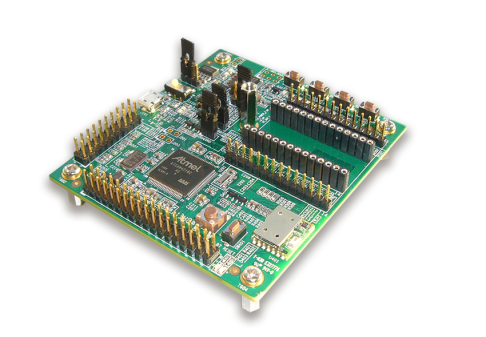
\includegraphics[width=0.50\textwidth]{coinesAPI_images/APP20-APP20.png}
			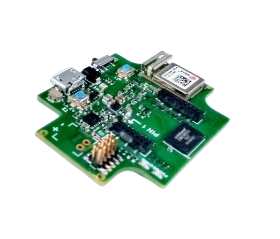
\includegraphics[width=0.40\textwidth]{coinesAPI_images/APP30.png}
			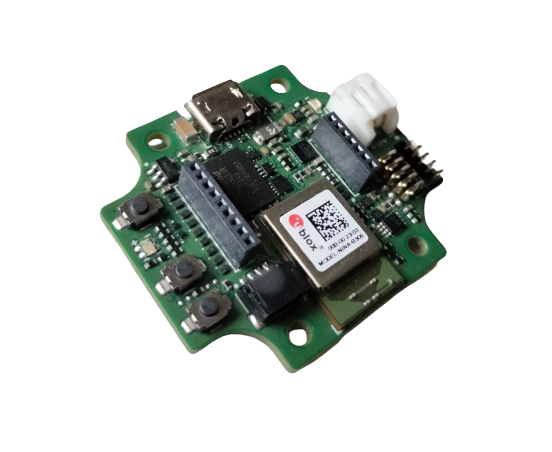
\includegraphics[width=0.40\textwidth]{coinesAPI_images/APP31.png}
			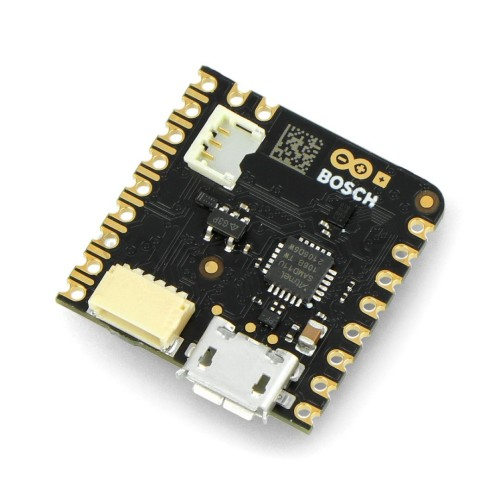
\includegraphics[width=0.40\textwidth]{coinesAPI_images/NiclaSenseME.jpg}
			\caption{Application Board 2.0/3.0/3.1/Nicla Sense ME}
		\end{center}
	\end{figure}

	\item \textbf{Sensor Shuttle board}: A sensor specific shuttle board also known as breakout board is a PCB with the sensor mounted on it. The shuttle board allows easy access to the sensor pins via a simple socket and can be directly plugged into the Bosch Sensortec’s Application boards. APP3.x shuttle boards also known as mini shuttle boards has smaller form factor when compared with APP2.0 shuttle board.
	
	\begin{figure}[H]
		\begin{center}
			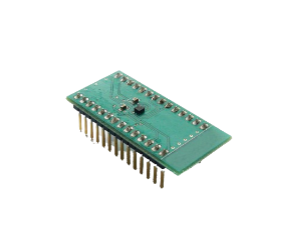
\includegraphics[width=0.35\textwidth]{coinesAPI_images/BMA222E_1.png}
			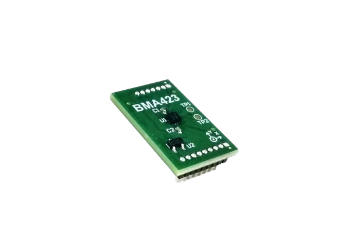
\includegraphics[width=0.45\textwidth]{coinesAPI_images/BMA423.png}
			\caption{APP2.0/3.x sensor shuttle board}
		\end{center}
	\end{figure}

	\item \textbf{COINES}: COINES provides a low-level interface for communication with Bosch Sensortec's Engineering boards enabling access to their MEMS sensors through sample applications and SensorAPI. For detailed description, refer to sections below.
\end{enumerate}

\newpage


\end{document}